\documentclass[tikz,border=7pt]{standalone}
\usepackage{amsmath,amssymb}
\usetikzlibrary{calc}

\begin{document}
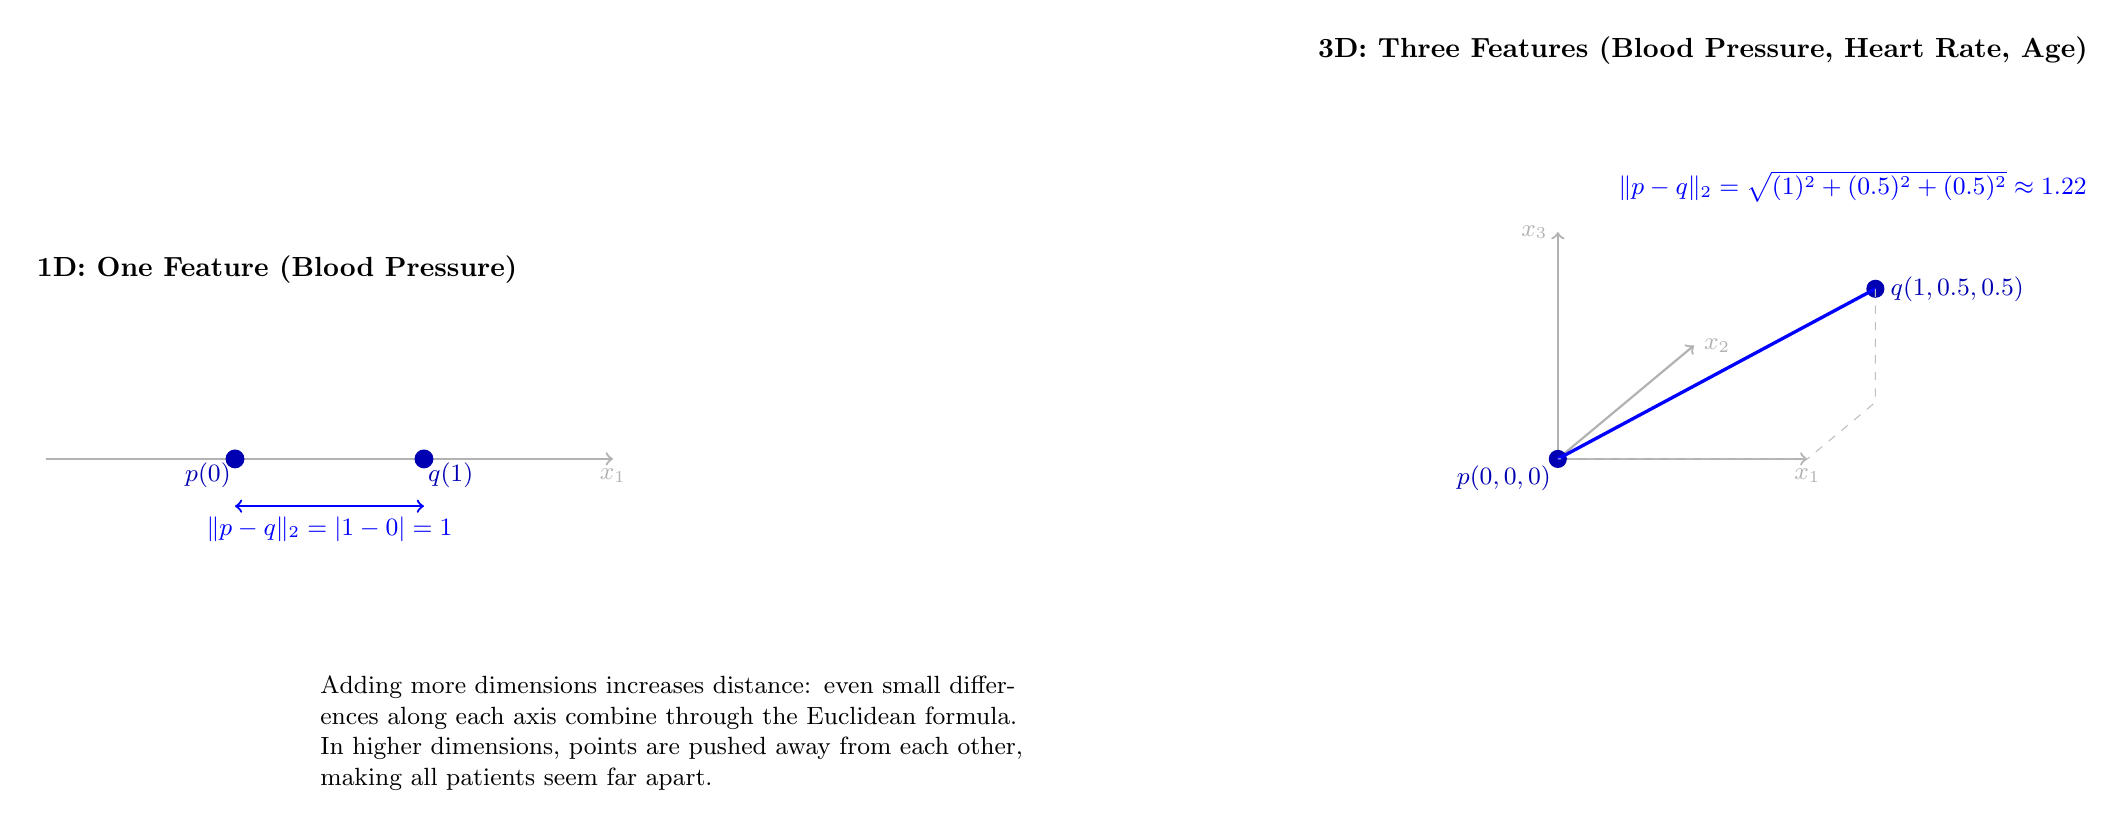
\begin{tikzpicture}[scale=2.4, every node/.style={font=\small}]

% ---------- 1D PANEL ----------
\begin{scope}[xshift=-1.5cm]
  \node[anchor=west,font=\bfseries] at (-1.1,1.0) {1D: One Feature (Blood Pressure)};
  % Axis
  \draw[->,gray!60,thick] (-1.0,0) -- (2.0,0) node[below] {$x_1$};
  % Points
  \fill[blue!70!black] (0,0) circle (0.05) node[below left=-2pt] {$p(0)$};
  \fill[blue!70!black] (1.0,0) circle (0.05) node[below right=-2pt] {$q(1)$};
  % Distance arrow
  \draw[<->,blue,thick] (0,-0.25) -- (1.0,-0.25)
    node[midway,below] {$\|p-q\|_2 = |1-0| = 1$};
\end{scope}

% ---------- 3D PANEL ----------
\begin{scope}[xshift=5.5cm,scale=1.2]
  \node[anchor=west,font=\bfseries] at (-1.1,1.8) {3D: Three Features (Blood Pressure, Heart Rate, Age)};
  % Axes
  \coordinate (O) at (0,0);
  \coordinate (E1) at (1.1,0.0);
  \coordinate (E2) at (0.6,0.5);
  \coordinate (E3) at (0.0,1.0);
  \draw[->,gray!60,thick] (O)--(E1) node[below] {$x_1$};
  \draw[->,gray!60,thick] (O)--(E2) node[right] {$x_2$};
  \draw[->,gray!60,thick] (O)--(E3) node[left] {$x_3$};

  % Points
  \coordinate (p) at (O);
  \coordinate (q) at ($(O)+1.0*(E1)+0.5*(E2)+0.5*(E3)$);
  \fill[blue!70!black] (p) circle (0.04) node[below left=-1pt] {$p(0,0,0)$};
  \fill[blue!70!black] (q) circle (0.04) node[right=2pt] {$q(1,0.5,0.5)$};

  % 3D line
  \draw[very thick,blue] (p)--(q);

  % Dashed projections
  \coordinate (q_xy) at ($(O)+1.0*(E1)+0.5*(E2)$);
  \coordinate (q_x)  at ($(O)+1.0*(E1)$);
  \draw[dashed,gray!50] (q)--(q_xy)--(q_x)--(p);

  % Formula
  \node[blue] at (1.3,1.2)
    {$\|p-q\|_2 = \sqrt{(1)^2 + (0.5)^2 + (0.5)^2} \approx 1.22$};

\end{scope}

% ---------- EXPLANATION ----------
\node[align=left, text width=9cm, anchor=north west, font=\small] at (-1.1,-1.1)
{Adding more dimensions increases distance: even small differences along each axis combine
through the Euclidean formula. In higher dimensions, points are pushed away from each other,
making all patients seem far apart.};

\end{tikzpicture}
\end{document}
